\section{Application à un drive oscillant}
\cite{mythesis} \cite{Shillito_2021} Un drive est une onde (un pulse) qu'on envoie sur un transmon (qubit) afin de manipuler son état. Ici, le drive oscille et cela occasionne des changements de niveaux d'énergie. Le qubit évolue donc avec un hamiltonien dépendant du temps.

\subsection{Dérivation}

\subsubsection{Préliminaires}
On considère un hamiltonien dépendant du temps de la forme 

\begin{equation}
    H(t) = H_0 + V(t)
\end{equation}

où $H_0 = \sum_{k} \lambda_k \ket{k}\bra{k}$ dans sa base d'états propres et $V(t) = X\cos(\omega t)$ pour un certain opérateur $X$. En décomposant le cosinus en exponentielles complexes, 

\begin{equation*}
    H(t) = H_0 + X\left(\frac{e^{i \omega t} + e^{-i\omega t}}{2}\right)
\end{equation*}

Pour une variation infime de temps et en utilisant la définition de (2.1), on trouve (et ce n'est pas très beau)

\begin{equation*}
    U(t+\delta t, t) = \sum_{n=0}^{\infty} (-i)^n \int_{t}^{t+\delta t}\int_{t}^{t_n}...\int_{t}^{t_2}H(t_n)...H(t_1)dt_1 ... dt_n
\end{equation*}
\begin{equation*}
    = \sum_{n=0}^{\infty} (-i)^n \int_{t}^{t+\delta t}\int_{t}^{t_n}...\int_{t}^{t_2}\left(H_0 + 
    V(t_n)\right)...\left(H_0 + V(t_1)\right)dt_1 ... dt_n
\end{equation*}
\begin{equation*}
    = \sum_{n=0}^{\infty} (-i)^n \int_{t}^{t+\delta t}\int_{t}^{t_n}...\int_{t}^{t_2} \left(H_0...H_0 + H_0...H_0V(t_1) + ... + V(t_n)H_0...H_0 + ... + V(t_n)...V(t_1)\right)dt_1 ... dt_n
\end{equation*}
\begin{equation}
    = \sum_{n=0}^{\infty} \int_{t}^{t+\delta t}\int_{t}^{t_n}...\int_{t}^{t_2} (-i)^n H_0...H_0 dt_1...dt_n + ... + \sum_{n=0}^{\infty} \int_{t}^{t+\delta t}\int_{t}^{t_n}...\int_{t}^{t_2}(-i)^n V(t_n)...V(t_1) dt_1...dt_n
\end{equation}

On peut voir que la distribution des termes correspond à l'ensemble des combinaisons de $n$ opérateurs où on choisit soit $H_0$ ou $V(t)$ pour chacun d'eux. Il y a donc au total $2^n$ termes chacun $n$ opérateurs pouvant alterner entre des suites de $H_0$ ou de $V(t)$ de différentes longueurs. Graphiquement, on peut représenter cela par la figure 2. On s'apprête maintenant à réécrire (2.2) différement et la dérivation pour y arriver peut facilement porter à confusion. On essaie d'expliquer le plus possible chaque étape.

\begin{figure}[H]
    \centering
     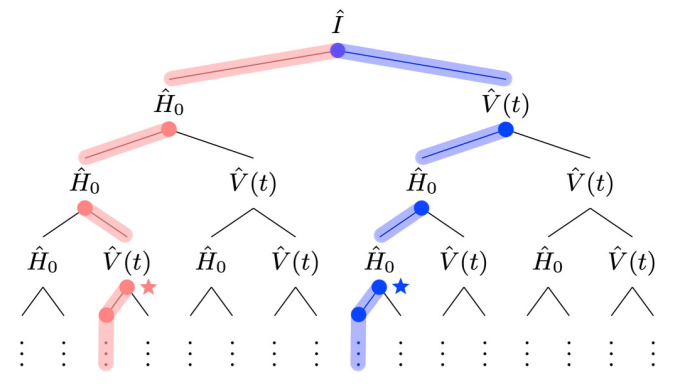
\includegraphics[width=0.45\textwidth]{images/ch2/embranchements.png}
    \caption{Arbre permettant de générer l'ensemble des combinaisons}
\end{figure}

\subsubsection{Dérivation (partie 1)}
On considère maintenant $n$ comme étant le nombre de $V(t)$ présents dans chaque terme de (2.2) et on omet temporairement les indices $V(t_j)$ pour éviter de se mélanger avec l'ancienne écriture. Il ne s'agit plus du même $n$ de (2.2) et il faut alors un nouveau moyen d'écrire tout cela avec ce changement de variables. Pour se faire, on introduit les $m_i$ qui indiquent combien d'applications de $H_0$ il y a avant une application de $V(t)$. Par exemple,

\begin{equation*}
    H_0V(t)H_0H_0 = (H_0)^1V(t)(H_0)^2 = (H_0)^{m_1}V(t)(H_0)^{m_0} \implies m_0 = 2, m_1 = 1
\end{equation*}
\begin{equation*}
    V(t)V(t) = (H_0)^0V(t)(H_0)^0V(t)(H_0)^0 \implies m_0 = m_1 = m_2 = 0
\end{equation*}

En général, ils sont indexés de $m_0$ à $m_n$, car pour un nombre $n$ de $V(t)$, on peut avoir jusqu'à $n+1$ blocs $H_0...H_0$ ayant des longueurs différentes.

\begin{equation*}
    \underline{H_0H_0}V(t) : \text{ 1 bloc, } \underline{H_0}V(t)\underline{H_0} : \text{ 2 blocs, } V(t)\underline{H_0H_0} : \text{ 1 bloc}
\end{equation*}



Cependant, chaque terme de (2.2) a une somme infinie. Ainsi, ces blocs peuvent être arbitrairement longs, faisant en sorte que les $m_i$ peuvent prendre des valeurs entre 0 et l'infini. Il est plus concis de les mettre dans un vecteur $\boldsymbol{m} = \left[m_n, ..., m_0\right] \in \mathbb{Z}^{n+1}_+$. Ainsi, on peut écrire toute chaîne d'opérateurs comme 

\begin{equation}
    (H_0)^{m_n}V(t)(H_0)^{m_{n-1}}V(t)...(H_0)^{m_1}V(t)(H_0)^{m_0}
\end{equation}

dont on obtient sa longueur $M$ (le nombre total d'opérateurs) grâce à 

\begin{equation}
    M = \left(\sum_{i=0}^{n}m_i\right) + n
\end{equation}

\subsubsection{Dérivation (partie 2)}
La prochaine étape est maintenant de retrouver les indices dans les $V(t)$ avec notre nouvelle notation. On sait déjà qu'il y aura $n$ opérateurs $V(t)$, mais on doit pouvoir retrouver leur positionnement dans la chaîne d'opérateurs. On peut simplement compter combien il y a de $H_0$ et d'autres $V(t)$ avant celui qui nous intéresse. Par exemple, pour $n=2$, on pourrait avoir la chaîne

\begin{equation*}
    H_0V(t)H_0V(t)H_0 \implies \boldsymbol{m} = \left[1, 1, 1\right]
\end{equation*}

Le premier $V(t)$ s'applique nécessairement après $m_0 = 1$ opérateur $H_0$. Le deuxième s'applique nécessairement après $m_0 = 1$ opérateur $H_0$, un $V(t)$ puis $m_1 = 1$ opérateur $H_0$. Si $p \in \left[1..n\right]$ est une variable qui passe au travers des $n$ opérateurs $V(t)$, alors il est facile de voir l'indexage $V(t_{l(p)})$ où

\begin{equation}
    l(p) = \left(\sum_{j=0}^{p-1}m_j\right) + p
\end{equation}

Pour reprendre l'exemple, on aurait 

\begin{equation*}
    H_0V(t_{l(2)})H_0V(t_{l(1)})H_0 = H_0V(t_{m_1 + m_0 + 2})H_0V(t_{m_0 + 1})H_0 = H_0V(t_4)H_0V(t_2)H_0
\end{equation*}

ce qui est exactement comme dans (2.2).

\subsubsection{Dérivation (partie 3)}
Ensuite, on étend les $V(t_{l(p)})$ selon leur définition qu'on rappelle ici.

\begin{equation*}
    V(t_{l(p)}) = X\left(\frac{e^{i\omega t_{l(p)}} + e^{-i\omega t_{l(p)}}}{2}\right)
\end{equation*}

Toujours avec le même exemple,

\begin{equation*}
    H_0V(t_4)H_0V(t_2)H_0 = \left(\frac{e^{i\omega t_4} + e^{-i\omega t_4}}{2}\right)\left(\frac{e^{i\omega t_2} + e^{-i\omega t_2}}{2}\right)H_0XH_0XH_0 
\end{equation*}
\begin{equation*}
    = \frac{1}{2^2}\left(e^{i\omega t_2}e^{i\omega t_4} + e^{i\omega t_2}e^{-i\omega t_4} + e^{-i\omega t_2}e^{i\omega t_4} + e^{-i\omega t_2}e^{-i\omega t_4}\right)H_0XH_0XH_0
\end{equation*}

On introduit maintenant le vecteur à $n$ dimensions $\boldsymbol{\omega}_n$ dont chacun de ses éléments peut soit être $+\omega$ ou $-\omega$. On peut aller chercher l'élément $i$ par $\boldsymbol{\omega}_n[i]$. Pour un $n$ donné, on voit qu'il en existe $2^n$ différents qu'on rassemble dans $\left\{\boldsymbol{\omega}_n\right\}$. Notamment, 

\begin{equation*}
    \left\{\boldsymbol{\omega}_2\right\} = \left\{\left[+\omega, +\omega\right], \left[+\omega, -\omega\right], \left[-\omega, +\omega\right], \left[-\omega, -\omega\right]\right\}    
\end{equation*}

On peut alors réécrire le produit d'exponentielles comme

\begin{equation*}
    \frac{1}{2^2}\sum_{\left\{\boldsymbol{\omega}_2\right\}}\left(\prod_{p=1}^{2}e^{i\boldsymbol{\omega}_2[p]t_{l(p)}} H_0XH_0XH_0\right)
\end{equation*}

Ainsi, (2.3) peut être réécrit de la manière suivante.

\begin{equation}
    \frac{1}{2^n}\sum_{\left\{\boldsymbol{\omega}_n\right\}}\left(\prod_{p=1}^{n}e^{i\boldsymbol{\omega}_n[p]t_{l(p)}} (H_0)^{m_n}X ... X(H_0)^{m_0}\right)
\end{equation}

\subsubsection{Dérivation (partie 4)}
Il est maintenant temps de remettre les précédentes parties dans le contexte de (2.2). D'abord, on se retrouve avec

\begin{equation*}
    \int_{t}^{t + \delta t}\int_{t}^{t_M}...\int_{t}^{t_2} (-i)^M \left(\frac{1}{2^n}\sum_{\left\{\boldsymbol{\omega}_n\right\}}\left(\prod_{p=1}^{n} e^{i\boldsymbol{\omega}_n[p]t_{l(p)}} (H_0)^{m_n}X...X(H_0)^{m_0}\right)\right)dt_1 ... dt_M
\end{equation*}
\begin{equation*}
    = \frac{1}{2^n}\sum_{\left\{\boldsymbol{\omega}_n\right\}}\left(\int_{t}^{t + \delta t}\int_{t}^{t_M}...\int_{t}^{t_2} (-iH_0)^{m_n}X...X(-iH_0)^{m_0} \cdot (-i)^n \prod_{p=1}^{n}e^{i\boldsymbol{\omega}_n[p]t_{l(p)}} dt_1 ... dt_M\right)
\end{equation*}

Il y a ensuite une somme infinie pour chaque terme qu'on absorbe dans les différentes longueurs $m_i$. On doit donc ajouter

\begin{equation*}
    \frac{1}{2^n}\sum_{\left\{\boldsymbol{\omega}_n\right\}}\sum_{\boldsymbol{m} \in \mathbb{Z}^{n+1}_+}\left(\int_{t}^{t + \delta t}\int_{t}^{t_M}...\int_{t}^{t_2} (-iH_0)^{m_n}X...X(-iH_0)^{m_0} \cdot (-i)^n \prod_{p=1}^{n}e^{i\boldsymbol{\omega}_n[p]t_{l(p)}} dt_1 ... dt_M\right)
\end{equation*}

Puis, on doit sommer la précédente équation pour tous les nombres $n$ de $V(t)$.

\begin{equation*}
    U(t+\delta t, t) = \sum_{n=0}^{\infty}\sum_{\left\{\boldsymbol{\omega}_n\right\}}\frac{1}{2^n}\sum_{\boldsymbol{m} \in \mathbb{Z}^{n+1}_+}\left(\int_{t}^{t + \delta t}\int_{t}^{t_M}...\int_{t}^{t_2} (-iH_0)^{m_n}X...X(-iH_0)^{m_0} \cdot (-i)^n \prod_{p=1}^{n}e^{i\boldsymbol{\omega}_n[p]t_{l(p)}} dt_1 ... dt_M\right)
\end{equation*}

\subsubsection{Dérivation (dernière partie)}
Finalement, on procède simplement à un changement de variables $t_i^{'} = t_i - t$. Ainsi, 

\begin{equation*}
    dt_i^{'} = dt_i - dt = dt_i    
\end{equation*}
\begin{equation*}
    t_i = t_i^{'} + t
\end{equation*}
\begin{equation*}
    t_i \in \left[t, t_j\right] \implies t_i^{'} \in [0, t_j^{'}]
\end{equation*}

nous donnent tout ce qu'il faut pour faire le changement de variables.

\begin{equation*}
    U(t+\delta t, t) = \sum_{n=0}^{\infty}\sum_{\left\{\boldsymbol{\omega}_n\right\}}\frac{1}{2^n}\sum_{\boldsymbol{m} \in \mathbb{Z}^{n+1}_+}\left(\int_{0}^{\delta t}\int_{0}^{t_M^{'}}...\int_{0}^{t_2^{'}} (-iH_0)^{m_n}X...X(-iH_0)^{m_0} \cdot (-i)^n \prod_{p=1}^{n}e^{i\boldsymbol{\omega}_n[p](t_{l(p)}^{'} + t)} dt_1^{'} ... dt_M^{'}\right)
\end{equation*}
\begin{equation*}
    = \sum_{n=0}^{\infty}\sum_{\left\{\boldsymbol{\omega}_n\right\}}\left(\prod_{p=1}^{n}e^{i\boldsymbol{\omega}_n[p]t}\right)\frac{1}{2^n}\sum_{\boldsymbol{m} \in \mathbb{Z}^{n+1}_+}\left(\int_{0}^{\delta t}\int_{0}^{t_M^{'}}...\int_{0}^{t_2^{'}} (-iH_0)^{m_n}X...X(-iH_0)^{m_0} \cdot (-i)^n \prod_{p=1}^{n}e^{i\boldsymbol{\omega}_n[p]t_{l(p)}^{'}} dt_1^{'} ... dt_M^{'}\right)
\end{equation*}
\begin{equation*}
    = \sum_{n=0}^{\infty}\sum_{\left\{\boldsymbol{\omega}_n\right\}}e^{i\sum_{p=1}^{n}\boldsymbol{\omega}_n[p]t}\frac{1}{2^n}\sum_{\boldsymbol{m} \in \mathbb{Z}^{n+1}_+}\left(\int_{0}^{\delta t}\int_{0}^{t_M^{'}}...\int_{0}^{t_2^{'}} (-iH_0)^{m_n}X...X(-iH_0)^{m_0} \cdot (-i)^n \prod_{p=1}^{n}e^{i\boldsymbol{\omega}_n[p]t_{l(p)}^{'}} dt_1^{'} ... dt_M^{'}\right)
\end{equation*}

Ce n'est pas très beau, alors on définit

\begin{equation}
    S^{(n)}_{\boldsymbol{m}}(\boldsymbol{\omega}_n, \delta t) = \int_{0}^{\delta t}\int_{0}^{t_M^{'}}...\int_{0}^{t_2^{'}} (-iH_0)^{m_n}X...X(-iH_0)^{m_0} \cdot (-i)^n \prod_{p=1}^{n}e^{i\boldsymbol{\omega}_n[p]t_{l(p)}^{'}} dt_1^{'} ... dt_M^{'}
\end{equation}
\begin{equation}
    S^{(n)}(\boldsymbol{\omega}_n, \delta t) = \frac{1}{2^n}\sum_{\boldsymbol{m} \in \mathbb{Z}^{n+1}_+} S^{(n)}_{\boldsymbol{m}}(\boldsymbol{\omega}_n, \delta t)
\end{equation}
\begin{equation}
    U^{(n)}(t + \delta t, t) = \sum_{\left\{\boldsymbol{\omega}_n\right\}}e^{i\sum_{p=1}^{n}\boldsymbol{\omega}_n[p]t}S^{(n)}(\boldsymbol{\omega}_n, \delta t)
\end{equation}

de sorte que 

\begin{equation}
    U(t+\delta t, t) = \sum_{n=0}^{\infty}U^{(n)}(t+\delta t, t)
\end{equation}

La transformation est assez exotique comme on vient de le voir.

\subsection{Ordre 0}

\subsection{Ordre 1}

